%% Governed feature selection for credit-risk models — IEEE TAI submission
%% Build: run build.ps1 (closes Acrobat if it holds the PDF, compiles, reopens).
%% Manual: latexmk -pdf main.tex
% IEEE TAI SUBMISSION format: 9pt, two-column (house style).
% (For an easier-to-read single-column review draft, use [11pt,journal,onecolumn].)
\documentclass[9pt,journal]{IEEEtai}

\usepackage[utf8]{inputenc}
\usepackage[T1]{fontenc}
\usepackage{amsmath,amssymb}
\usepackage{graphicx}
\usepackage{booktabs}
\usepackage{array}
\usepackage{url}
\usepackage{xcolor}
\usepackage{tikz}
\usetikzlibrary{arrows.meta,positioning,calc}
\usepackage{algorithm}
\usepackage{algpseudocode}
\usepackage[hidelinks]{hyperref}

% ---- metadata ----
\title{Governed Feature Selection for Credit-Risk Models: Shapley Attribution with Pre-Registered Parsimony under a Decision-Gate Governance Framework}

\author{Ravi\IEEEauthorrefmark{1}
\thanks{\IEEEauthorrefmark{1}The author is with the Indian Institute of Foreign Trade, New Delhi, India (e-mail: ravi\_phdm23@iift.edu).}
\thanks{Manuscript prepared \today. This is a working draft for internal review, not a submitted version.}}

\markboth{IEEE Transactions on Artificial Intelligence, Vol.~XX, No.~XX, 2027}%
{Ravi: Governed Feature Selection for Credit-Risk Models}

\begin{document}
\maketitle

\begin{abstract}
Machine-learning credit-risk models are increasingly accurate but remain hard to
\emph{govern}: the questions of \emph{which} features are genuinely useful, \emph{how
parsimonious} a defensible model may be, and \emph{whether} a selection is adequately
powered and fair are usually answered by analyst judgement rather than a reproducible,
auditable procedure. We present two coupled contributions. The first is a pre-registered
feature-selection methodology that separates order-invariant \emph{attribution} (sampled
Shapley importance against a shadow-feature null) from a distinct, fixed \emph{selection}
rule (the smallest feature set that is both DeLong-indistinguishable from the full model and
within a 5\% relative-Gini tolerance), followed by always-on isotonic calibration and a
regulatory PD floor. The second is a hash-chained decision-gate governance framework
(G0--GF) that wraps it with materiality-tiered rigour, binding every statistical bar to a
cited source and separating \emph{governance} decisions from \emph{analytics} parameters,
which are never re-opened. Across a corpus of
fourteen public and reference credit datasets run under one fixed configuration, we show that
the same rule yields genuine parsimony at small sample sizes yet near-full feature sets at
large ones (a large-$N$ sensitivity effect we characterise), that excluding a protected
attribute is necessary but not sufficient to remove disparate impact, and that signal
strength---not sample size---sets the achievable discrimination ceiling. We add the Riley
\emph{et al.} minimum-sample-size calculation alongside events-per-variable as a reported
sufficiency diagnostic and give a retrospective across the corpus.
\end{abstract}

\begin{IEEEImpStatement}
Credit decisions affect access to capital for individuals and firms, and supervisors now
require model-risk controls (e.g., the U.S.\ interagency guidance superseding SR~11-7, and
the EU AI Act's treatment of creditworthiness assessment as high-risk). This work shows how
feature selection---an early, consequential step usually left to discretion---can be made
\emph{reproducible and auditable} without inventing economic assumptions: thresholds and
pricing remain institution inputs, and governance gates decide process, not analytics. The
framework makes a model's parsimony, calibration, fairness, and data-sufficiency claims
traceable to recorded runs and cited bars, which should lower the cost of independent
validation and reduce the risk of overstated or unfair models reaching deployment.
\end{IEEEImpStatement}

\begin{IEEEkeywords}
Credit risk, feature selection, Shapley values, model governance, calibration, fairness,
disparate impact, sample size, explainable AI.
\end{IEEEkeywords}

\section{Introduction}
\IEEEPARstart{M}{achine}-learning models now dominate credit-risk scoring, yet their
\emph{governance} has not kept pace with their accuracy. A modern scorecard is the product of
dozens of consequential choices made before any headline metric is reported---which raw columns
to admit, how to bin and screen them, which to keep, how small a model is defensible, and whether
the data are even adequate to support it. In practice these choices are made by analyst
judgement and documented, if at all, after the fact. That is precisely where model risk
concentrates, and precisely what supervisors now scrutinise: the U.S.\ interagency guidance
SR~26-2 (superseding SR~11-7) demands effective, independent challenge of model development; the
EU AI Act classifies creditworthiness assessment as high-risk; and Basel CRE36 requires a use
test and a per-grade calibration backtest. None of these tells a practitioner \emph{how} to make
the early modelling steps reproducible and auditable.

We identify three governance gaps in the feature-selection stage. First, \textbf{which features
are genuinely useful}: greedy, order-dependent screening produces artefactual retention, and
Shapley-style attribution---increasingly the default interpretability tool---fairly apportions
importance but does not, by itself, select a subset. Second, \textbf{how parsimonious a model may
defensibly be}: small differences in discrimination are routinely presented as wins or losses
with no inferential test, and the ``right'' number of features is asserted rather than derived.
Third, \textbf{whether the data are adequate and the model fair}: sample-size justification
rarely goes beyond a rule of thumb, and the removal of a protected attribute is often assumed to
remove disparate impact. Each gap is an opening for an overstated or unfair model to reach
deployment with a clean-looking paper trail.

We address these with two coupled artefacts. The first is a \emph{pre-registered
feature-selection methodology} that cleanly separates order-invariant \emph{attribution} from a
fixed \emph{selection} rule, tests feature signal against an empirical shadow-feature null,
calibrates by construction, and reports both events-per-variable and the Riley minimum sample
size as governed sufficiency diagnostics. The second is a \emph{decision-gate governance
framework} that wraps the methodology in a materiality-tiered sequence of gates, each closing
with an accountable human sign-off written to a tamper-evident hash chain, and---by design---never
lets a per-run governance decision re-open a pre-registered analytical parameter.
Evaluated as a single fixed configuration across fourteen credit datasets, the pair exposes
behaviour that discretion would hide: the same selection rule yields genuine parsimony at small
$N$ but near-full feature sets at large $N$; excluding a protected attribute does not remove
disparate impact; and signal strength, not sample size, bounds achievable discrimination.

\textbf{Contributions.}
\begin{enumerate}
\item A \textbf{pre-registered feature-selection methodology} separating Shapley
\emph{attribution} from a fixed \emph{parsimony} selection rule (\S\ref{sec:sharp}).
\item A \textbf{hash-chained, materiality-tiered decision-gate governance framework} binding
every bar to a cited source and separating governance from analytics (\S\ref{sec:aegis}).
\item An empirical study over fourteen datasets under one fixed configuration, including the
large-$N$ parsimony effect, the ``necessary-but-not-sufficient'' fairness finding, and a
Riley-\emph{et al.}\ sample-size retrospective (\S\ref{sec:results}).
\end{enumerate}

\section{Related Work}\label{sec:related}
\textbf{Feature importance and selection.} Classical selection splits into filter methods
(e.g.\ Information Value, the credit-scoring standard \cite{siddiqi2006}), wrapper methods, and
embedded penalisation (LASSO, elastic net). Shapley-based attribution has become the dominant
interpretability tool: SHAP \cite{lundberg2017shap} gives local, per-prediction attributions,
while global measures such as SAGE \cite{covert2020sage} and the Shapley Population Variable
Importance Measure (SPVIM) \cite{williamson2020spvim} attribute model-level predictiveness. A
recurring confusion---which our methodology is built to avoid---is treating these attributions as a
\emph{selection} criterion: a Shapley value fairly \emph{apportions} predictiveness but does not
identify a minimal sufficient subset, so an importance ranking must be paired with an explicit
selection rule. Boruta's shadow-feature device \cite{kursa2010boruta} and stability selection
\cite{meinshausen2010stability} address the related problem of distinguishing real signal from
noise; our methodology adopts the shadow-null idea as its retention test.

\textbf{Parsimony and equivalence.} Preferring the smallest model statistically consistent with
the best one has a long heritage---the one-standard-error rule of CART \cite{breiman1984cart}
and its treatment in the statistical-learning literature \cite{hastie2009}. Our methodology operationalises
this with a paired-AUC equivalence test \cite{delong1988} plus a relative-Gini tolerance, rather
than an information criterion, because discrimination is the quantity credit practice cares about
\cite{lessmann2015,siddiqi2006}.

\textbf{Model-risk governance.} Supervisory expectations for model risk---the U.S.\ interagency
guidance SR~26-2 \cite{sr26_2} (superseding SR~11-7), Basel CRE36 \cite{bcbs_cre} (use test,
per-grade calibration backtest), the EU AI Act's \cite{euaiact2024} high-risk regime for
creditworthiness assessment, and the EBA's Margin-of-Conservatism guidance---specify \emph{what}
must be validated, documented, and independently
challenged, but not a concrete, reproducible procedure that couples feature selection to signed,
tamper-evident approval. Our governance framework fills that gap by turning each analytical stage into a governed
gate with a hash-chained decision log. Documentation artefacts such as model cards
\cite{mitchell2019modelcards} and datasheets for datasets \cite{gebru2021datasheets} standardise
\emph{what} to report about a model or data source, but they are descriptive records rather than a
gated, append-only decision process; our framework is complementary, producing such records as a
by-product of signed gate decisions.

\textbf{Fairness and disparate impact.} Anti-discrimination practice distinguishes disparate
\emph{treatment} from disparate \emph{impact}, the latter commonly screened with the four-fifths
rule (EEOC \cite{eeoc1978}). A substantial fairness-in-ML literature formalises group-fairness criteria
\cite{hardt2016eoo}; a consistent empirical lesson, which our runs reproduce, is that removing a
protected attribute is necessary but not sufficient, because correlated features reconstruct it.

\textbf{Sample-size adequacy.} Credit-scoring studies rarely report a sample-size justification
beyond the events-per-variable rule of thumb \cite{peduzzi1996}. Recent work shows EPV is too
coarse \cite{vansmeden2019} and derives signal-aware minimum sample sizes for prediction models
\cite{riley2019sim,riley2020bmj}, with a C-statistic-to-$R^2$ route for forward use
\cite{rileyvancalster2020}. Our methodology reports both EPV and the Riley minimum-$N$ as governed
diagnostics. In sum, each ingredient exists in isolation; our contribution is their coupling
into one pre-registered, reproducible, and auditable pipeline, evaluated here as a fixed-config
corpus.

\begin{figure*}[!t]
\centering
\footnotesize
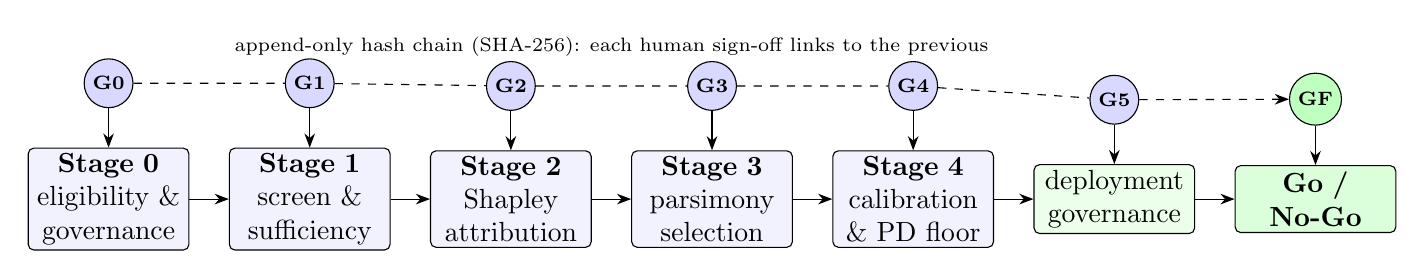
\begin{tikzpicture}[
  >={Stealth[length=1.8mm]},
  stage/.style={draw, rounded corners=2pt, minimum height=8.5mm, text width=19mm,
                align=center, fill=blue!5, inner sep=2pt},
  final/.style={draw, rounded corners=2pt, minimum height=8.5mm, text width=19mm,
                align=center, fill=green!8, inner sep=2pt},
  gate/.style={draw, circle, minimum size=6.2mm, inner sep=0pt, fill=blue!15,
               font=\scriptsize\bfseries},
  gatef/.style={draw, circle, minimum size=6.6mm, inner sep=0pt, fill=green!25,
               font=\scriptsize\bfseries}]
% pipeline stages
\node[stage] (s0) {\textbf{Stage 0}\\eligibility \& governance};
\node[stage, right=5mm of s0] (s1) {\textbf{Stage 1}\\screen \& sufficiency};
\node[stage, right=5mm of s1] (s2) {\textbf{Stage 2}\\Shapley attribution};
\node[stage, right=5mm of s2] (s3) {\textbf{Stage 3}\\parsimony selection};
\node[stage, right=5mm of s3] (s4) {\textbf{Stage 4}\\calibration \& PD floor};
\node[final, right=5mm of s4] (dep) {deployment governance};
\node[final, right=5mm of dep, fill=green!14] (gf) {\textbf{Go / No-Go}};
\foreach \a/\b in {s0/s1,s1/s2,s2/s3,s3/s4,s4/dep,dep/gf} \draw[->] (\a)--(\b);
% governance gates above each stage
\node[gate, above=5mm of s0] (g0){G0};
\node[gate, above=5mm of s1] (g1){G1};
\node[gate, above=5mm of s2] (g2){G2};
\node[gate, above=5mm of s3] (g3){G3};
\node[gate, above=5mm of s4] (g4){G4};
\node[gate, above=5mm of dep] (g5){G5};
\node[gatef, above=5mm of gf] (gfg){GF};
\foreach \g/\s in {g0/s0,g1/s1,g2/s2,g3/s3,g4/s4,g5/dep,gfg/gf} \draw[->] (\g)--(\s);
% hash-chained decision log linking the gates
\draw[dashed,->] (g0)--(g1)--(g2)--(g3)--(g4)--(g5)--(gfg);
\node[font=\scriptsize] at ($(g2)!0.5!(g3)+(0,5mm)$) {append-only hash chain (SHA-256): each human sign-off links to the previous};
\end{tikzpicture}
\caption{The governed pipeline. The feature-selection methodology (blue, Stages~0--4) runs under a
sequence of governance gates (G0--G5), each closed by an accountable human sign-off that is written
to an append-only hash chain; the committee gate GF rules the final Go/No-Go with all gate evidence
visible. Gates decide scope, eligibility, fairness treatment, cut-offs and disposition---never the
pre-registered analytical parameters (P8).}
\label{fig:pipeline}
\end{figure*}

\section{The Feature-Selection Methodology}\label{sec:sharp}
The proposed methodology deliberately separates two questions that are
routinely conflated in applied feature selection (the full pipeline and its governance gates are
shown in Fig.~\ref{fig:pipeline}):

\begin{itemize}
\item \textbf{Attribution} --- ``How much predictive value is attributable to this feature,
\emph{order-invariantly}?'' Answered by a Shapley importance measure against an empirical
null.
\item \textbf{Selection} --- ``What is the \emph{smallest} feature set whose performance is
statistically indistinguishable from the full set?'' Answered by a separate, pre-registered
stopping rule.
\end{itemize}

The separation is principled, not stylistic. Shapley values are a \emph{fair-attribution}
solution concept (efficiency, symmetry, dummy, additivity); they do not identify an optimal
subset. A redundant-but-informative feature still receives a positive share, and a feature
whose value concentrates in rare coalitions can average below any bar despite being needed.
Attribution therefore \emph{ranks}; a separately justified rule \emph{selects}. Greedy,
category-sequential screening---the common alternative---produces order-dependent, artefactual
retention; an order-invariant importance estimate plus an explicit selection rule avoids it.

\textbf{Inference target.} We estimate population feature importance \emph{with respect to a
specified learner and value function}: how much cross-validated predictiveness is recoverable
from a feature set, for a given learner class, on a given population---\emph{not} how much a
feature ``matters to credit risk'' in the abstract. Formally, with value function $v(S)$ equal
to the cross-validated predictiveness of the columns in $S$, the importance of feature $j$ is
the Shapley value
\begin{equation}
\phi_j \;=\!\!\sum_{S\subseteq N\setminus\{j\}}\!\!
\frac{|S|!\,(|N|-|S|-1)!}{|N|!}\,\bigl[v(S\cup\{j\})-v(S)\bigr],
\label{eq:shapley}
\end{equation}
which is the Shapley Population Variable Importance Measure (SPVIM) of Williamson and Feng
\cite{williamson2020spvim}. This is \emph{not} SAGE \cite{covert2020sage}, which marginalises
absent features out of a single fitted model; here each coalition $S$ is \emph{refit}.

The pipeline has five stages (0--4), summarised in Algorithm~\ref{alg:main}; the governance
framework that signs off on their outputs is described in \S\ref{sec:aegis}.

\begin{algorithm}[!t]
\caption{Governed feature selection (one dataset, fixed configuration)}
\label{alg:main}
\small
\begin{algorithmic}[1]
\Require data $(X,y)$; learner; value function $v$; shadows $m\!\ge\!10$;
tolerance $\tau{=}0.05$; level $\alpha{=}0.05$; confirmation threshold $c{=}0.80$; seed
\State screen features by $\mathrm{IV}\!\ge\!0.02$ with monotonic WOE binning \Comment{Stage 1}
\State group columns at $|\rho|\!\ge\!0.7$ into coalitional players $P$ \Comment{Stage 2}
\State add $m$ shadow players: row-permuted copies of real columns
\If{$|P|+m \le 15$}
  \State compute exact Shapley values $\phi$ for all players
\Else
  \State estimate $\phi$ by sampled permutations to a target MC s.e.
\EndIf
\State $b \gets$ 95th percentile of the shadow players' $\phi$ \Comment{empirical null}
\State $C \gets \{\,p : \phi_p > b \ \text{and bootstrap confirm.\ freq} \ge c\,\}$
\State rank $C$ by $\phi$ descending \Comment{Stage 3}
\For{$k=1,\dots,|C|$}
  \State fit top-$k$ on out-of-fold folds; record $\mathrm{Gini}_k$ and DeLong $p_k$ vs full
\EndFor
\State $k^\star \gets \min\{\,k : p_k\!\ge\!\alpha \ \text{and}\
  (\mathrm{Gini}_{\text{full}}\!-\!\mathrm{Gini}_k)/\mathrm{Gini}_{\text{full}}\!\le\!\tau\,\}$
\State calibrate the top-$k^\star$ model (isotonic); apply PD floor/cap \Comment{Stage 4}
\Ensure selected set (top-$k^\star$ of $C$), calibrated model, additive reason codes
\end{algorithmic}
\end{algorithm}

\subsection{Stage~0: Eligibility and data governance}
Stage~0 runs \emph{before any statistics}: it attaches a per-column classification that travels
with every downstream result, and excludes columns that cannot be modelled---leakage,
identifiers, constants and junk---each by a \emph{computable precondition} recorded with its
measured value (Table~\ref{tab:g0excl}), so every exclusion is reproducible. Protected and proxy
attributes, by contrast, are tagged rather than dropped: each is labelled
\texttt{permissible}, \texttt{prohibited} (e.g.\ sex, age, marital status), \texttt{proxy\_risk}
(e.g.\ geography, education, household composition), or \texttt{unclear}. On these public
research benchmarks, protected and proxy attributes are \emph{retained with mandatory
disclosure} so results remain comparable with the large published literature on the same
datasets; no model here is intended for live use. Stage~0 also records point-in-time
availability (flagging \texttt{near\_target} and \texttt{external\_score} columns that make a
model a behavioural or score-recovery exercise rather than an application scorecard), audits
sentinel codes and shared missingness for leakage, notes the accept-only sampling that
truncates feature distributions \cite{handhenley1997}, and declares \emph{mandatory} columns
and a missingness policy that are enforced only at scoring (\S\ref{sec:sharp}-F).
Two further Stage-0 \emph{reports} were added with the staged protocol (\S\ref{sec:staged}); neither
excludes a column or adds a pass/fail bar. A \emph{blank-versus-outcome scan} gives, for every column
with blanks, the share blank, the event rate among blank and among filled rows, and a Fisher exact
$p$-value against a Bonferroni reference. A \emph{look-ahead scan} flags column definitions containing
a temporal phrase (e.g.\ ``in 3 years'') so that a human reads them against the question of whether
they could use information after the statement date, and records a verdict.

\begin{table}[!t]
\centering
\caption{Stage-0 eligibility exclusions. Each is driven by a computable precondition; the
semantic categories pair that signal with a recorded rationale, never a silent drop. Examples
from the SBA run.}
\label{tab:g0excl}
\footnotesize
\begin{tabular}{@{}p{0.17\linewidth}p{0.47\linewidth}p{0.24\linewidth}@{}}
\toprule
Category & Computable precondition & Example (SBA) \\
\midrule
Constant & $\mathrm{nunique}\le1$ (zero variance) & \texttt{State}, \texttt{BalanceGross} \\
Identifier / PII & cardinality $\to n$ (a key), or high-cardinality free text & \texttt{LoanNr} (2102/2102), \texttt{Name} \\
Leakage & target agreement $\to 1$, or sentinel event-rate lift $\ge 3\times$; confirmed post-outcome by meaning & \texttt{MIS\_Status} ($100\%$), \texttt{ChgOffPrinGr} ($99.5\%$) \\
Junk & $\mathrm{isna().all()}$ (all-blank), or absent from the data dictionary & \texttt{xx} \\
\bottomrule
\end{tabular}
\end{table}

\subsection{Stage~1: Univariate screening}
Information Value (IV) is the single a-priori screen, at the conventional
threshold $\mathrm{IV}\ge0.02$ \cite{siddiqi2006}; Cram\'er's $V$, $\chi^2$ and $p$-values are
reported descriptively and decide nothing. Binning is monotonic Weight-of-Evidence (WOE) with
a minimum bin size of 5\% of rows,
\begin{equation}
\mathrm{WOE}_i=\ln\!\frac{g_i/G}{b_i/B},\qquad
\mathrm{IV}=\sum_i\Bigl(\tfrac{g_i}{G}-\tfrac{b_i}{B}\Bigr)\mathrm{WOE}_i,
\label{eq:woe}
\end{equation}
where $g_i,b_i$ are goods/bads in bin $i$. Monotonicity is enforced only where it is supported:
a genuinely U-shaped feature whose IV recovers $\ge20\%$ when the constraint is freed is tagged
\texttt{shape\_nonmonotonic} and routed to a single-column model check rather than being judged
on its monotonic IV. A reliability gate ($\chi^2$ minimum expected cell $\ge5$) and a
bin-count sensitivity check (WOE vs 5/10/20 quantile bins) escalate borderline columns to the
same model check, whose verdict is a Gini confidence interval excluding zero.

\subsection{Stage~2: Order-invariant attribution}
The default value function is repeated cross-validated AUC and the default learner is a
penalised logistic model on monotonic-WOE inputs (\texttt{woe\_logistic})---the credit-scoring
standard form: deterministic and hyperparameter-insensitive, which removes refit noise from
the Shapley estimate. No second learner is run in the governed process: the same learner is used for screening,
attribution, selection, calibration and deployment, so the model that is selected is the model that is calibrated and
scored. Class reweighting is \emph{off} by default: on GMSC it inflated the mean predicted probability
to $0.286$ against a true base rate of $0.067$, and the resulting miscalibration is avoided
rather than repaired.

Two devices make the attribution both tractable and honest. First, correlated columns are not
pruned (which would reintroduce a greedy univariate criterion); instead, hierarchical
clustering on $1-|\rho_{\text{Spearman}}|$ cut at $|\rho|=0.7$ makes \emph{each cluster a single
Shapley player}, preserving the efficiency property over the full candidate set. Second---the
central methodological fix---significance testing of Shapley values is replaced by a
\textbf{shadow-feature null} \cite{kursa2010boruta}: at least ten shadow players (row-permuted
copies of real columns) are added, the identical Shapley computation is run over the augmented
set, and a real player is \texttt{importance\_confirmed} only if its value exceeds the
$95^{\text{th}}$ percentile of the shadow distribution \emph{and} its bootstrap confirmation
frequency is $\ge0.80$. The bar is a quantile of an empirical null, so no multiple-testing
correction is needed and fold-dependence does not bias it. Benjamini--Hochberg \cite{bh1995} $p$-values and
Cohen's $d$ \cite{cohen1988} are retained only as reported diagnostics---usefully self-refuting, since on German
Credit a permuted-noise shadow column received $p=0.0000$ with a \emph{negative} Shapley value,
which a significance rule would have confirmed and the shadow bar correctly rejected.
Enumeration is exact when the player count (including shadows) is $\le15$ and sampled otherwise,
with the Monte Carlo standard error reported per player.

\subsection{Stage~3: Pre-registered parsimony}
The eligible set is the confirmed players, ranked by $\phi_j$. For $k=1,\dots,K$ the model on
the top-$k$ players is scored on \emph{out-of-fold} predictions (so every $k$ is evaluated on
the same rows and DeLong's paired test is valid \cite{delong1988}), and the full parsimony
curve is a required output. The stopping rule is fixed in advance: choose the smallest $k$ that
is both statistically indistinguishable from the full-candidate model by DeLong's test at
$\alpha=0.05$ \emph{and} within a relative-Gini tolerance,
\begin{equation}
k^\star=\min\Bigl\{k:\; p_{\text{DeLong}}(k)\ge0.05 \;\wedge\;
\tfrac{\mathrm{Gini}_{\text{full}}-\mathrm{Gini}_k}{\mathrm{Gini}_{\text{full}}}\le 0.05\Bigr\}.
\label{eq:stop}
\end{equation}
If no $k$ qualifies, that is reported as the result (``no parsimonious subset meets the
tolerance'')---it is never replaced by the best available $k$. Because the two conditions are
combined by \emph{and}, the rule behaves very differently across sample sizes (\S\ref{sec:results}):
at small $N$ both clear together and yield genuine parsimony, whereas at large $N$ DeLong detects
the loss from dropping even a weak feature and the full set is returned.

\subsection{Stage~4: Calibration, reason codes, and sufficiency diagnostics}
The selected model is calibrated by cross-validated isotonic regression \cite{zadrozny2002,niculescu2005} (always on), and
calibrated probabilities are used whenever a PD is quoted to a person. Because the learner is
WOE-logistic, the score is an exact additive decomposition
$\operatorname{logit}=\beta_0+\sum_j\beta_j\,\mathrm{WOE}_j(x)$, giving faithful per-feature
\emph{reason codes} with no post-hoc approximation. A regulatory PD floor of $0.03\%$ (Basel
CRE32.3) and a $99.9\%$ cap are applied at scoring, as are the Stage-0 mandatory-field gate and
missingness policy. Finally, data sufficiency is reported---never used to auto-reject---through
two diagnostics side by side: events-per-variable \cite{peduzzi1996,vansmeden2019} and the
Riley \emph{et al.}\ minimum sample size \cite{riley2020bmj,riley2019sim}, the latter derived
from the anticipated $C$-statistic and prevalence via the Cox--Snell $R^2$ approximation of
\cite{rileyvancalster2020}. A shortfall is a disclosed caveat the governance layer weighs, not
a gate failure---consistent with the principle that selection parameters are fixed and only
governance decides disposition.

\section{The Governance Framework}\label{sec:aegis}
The methodology of \S\ref{sec:sharp} produces a defensible \emph{model}; it does not, by itself, produce a defensible
\emph{decision to use that model}. A supervisor or internal audit function asks questions the
analytics cannot answer: who decided the data were adequate, and could they have decided
otherwise? Who chose this feature set, on what recorded rationale? Who is accountable if the
model is wrong, and were they independent of the builder? Where is the evidence that each
regulatory expectation was \emph{met}, not merely claimed? The governance framework answers these
by turning each methodology stage into a
\emph{governed decision gate}: the machine emits a recommendation and a full evidence pack, a
human with the right role and sufficient independence chooses from a closed set of genuinely
viable options, and the choice is written to a tamper-evident log. This mirrors modern
model-risk expectations---the U.S.\ interagency guidance SR~26-2 (superseding SR~11-7), the EU
AI Act's treatment of creditworthiness assessment as high-risk, and Basel CRE36---without
importing their numeric bars by assumption: every threshold used is tied to a cited source.

\subsection{Design principles}
Eight principles govern the framework; three are load-bearing. \textbf{(P1) Machine recommends,
human decides, record proves}: every gate is recommendation + evidence pack + closed options +
accountable sign-off + log entry. \textbf{(P2) Segregation of duties}: the Develop, Validate,
and Approve functions are never held by one person for one model. \textbf{(P8) Gates decide
governance, not analytics}: a gate's option set may \emph{never} re-open a pre-registered
analytical parameter (estimator mode, selection tolerances, shadow-bar quantile, confirmation frequency,
\texttt{random\_state}, CV folds). Those are fixed in the methodology, identical across every
dataset, and chosen once; gates decide scope, eligibility, fairness treatment, cutoffs, and
Go/No-Go. P8 is what keeps the method reportable: letting a per-run gate switch the estimator
would be the dataset-dependent, path-changing behaviour a research methodology must avoid. The
single failure mode the framework is explicitly designed against is \emph{rubber-stamping}---hence the
anti-strawman rule below and the independence requirements in \S\ref{sec:aegis}-E.

\subsection{The decision gates G0--GF}
The methodology's stages become gates G0--G5, with a final committee gate GF (Table~\ref{tab:gates}).
G0--G5 are \emph{stage gates} (a single accountable role signs each); GF is the \emph{committee
gate}, ruled by the Model Approval Committee. Crucially, GF is last and is decided only after
G4's per-grade calibration backtest and G5's cutoff policy and acceptance demonstration are
complete and visible---one does not approve deployment and then check whether the PDs are
honest and the decisions sensible.

\begin{table}[!t]
\centering
\caption{The decision gates and the methodology stage each governs.}
\label{tab:gates}
\footnotesize
\begin{tabular}{@{}llp{0.52\linewidth}@{}}
\toprule
Gate & Stage & Core question decided \\
\midrule
G0 & Stage 0 & Is the dataset fit to build on? (coverage, label integrity, scope) \\
G1 & Stage 1 & Which features survive screening; is $N$ adequate (EPV + Riley, reported)? \\
G2 & Stage 2 & Is the attribution stable enough to select on? \\
G3 & Stage 3 & Which feature set is adopted---parsimonious vs full, and the trade-off? \\
G4 & Stage 4 & Calibrated, discriminating, and fair enough to approve? (per-grade backtest) \\
G5 & Scoring & Deployment controls + cutoff policy + acceptance demonstration \\
GF & whole model & GO / GO-WITH-CONDITIONS / NO-GO (committee) \\
\bottomrule
\end{tabular}
\end{table}

A model is assigned a \emph{materiality tier} (HIGH / MEDIUM / LOW) at G0, after SR~26-2's
exposure-$\times$-purpose logic; the tier sets \emph{who} signs each gate and \emph{how high the
pass-bar sits}, but never changes the analytics---every metric is measured identically across
datasets. Lowering a tier is itself a recorded G0 decision.

\subsection{Staged execution: each stage stops at its gate}\label{sec:staged}
The gates of Table~\ref{tab:gates} could be walked after the whole pipeline has run, which is how the
fourteen corpus runs were executed (\S\ref{sec:setup}). That order has a cost: if an early gate changes
direction, the later stages have already been computed, and the signer has seen downstream numbers
before deciding upstream gates. The staged protocol removes both problems. Each methodology stage
runs, then \emph{stops at its gate}; the next stage starts only after the accountable role has chosen
an option, given a rationale of at least twenty characters, and the entry has been appended to the hash
chain. A gate cannot be sealed before its stage has run, and a stage refuses to run while the previous
gate is unsealed. A gate that changes direction at G0--G3 voids its own entry and every later one (kept
in the audit trail) and re-runs from the stage it governs; a change at G4, G5 or GF needs no re-run of the
methodology. The staged run calls the same primitives with the same arguments and seed as the one-shot
pipeline, and an all-approved staged run reproduces the one-shot candidates, selected columns, parsimony
curve, shadow bar, calibration and backtest (an automated equivalence test). Consequently P8 is unaffected:
staging changes \emph{when} a human decides, never \emph{what} is computed.

Three further changes move an assessment earlier rather than adding a bar. Events-per-variable and the
Riley minimum $N$ are reported on every basis reached (candidate columns, confirmed players, selected
model) at G1, G2 and G3. The regulatory acceptance checklist (rows R1--R10) is derived as evidence
appears, so the final gate reads a completed checklist; derived statuses are proposals that the signer
may override with a recorded note. And the holders of the signing roles are declared at G0, so that one
person holding several roles is visible when it occurs and not only at GF. At G5 the acceptance pack is
accompanied by a coverage report of which scoring controls the data actually exercises.

\subsection{Anatomy of a gate}
Each gate produces one Gate Decision Record with five parts: (i) the machine recommendation and
its numeric basis; (ii) the full evidence pack (the actual numbers, traceable to a run, not a
summary); (iii) a closed set of 2--4 options, each carrying its own data, rationale, benefits,
risks, and an explicit \emph{residual-risk acceptance}; (iv) a human sign-off (role, identity,
exactly one option, free-text rationale, timestamp); and (v) an append-only log entry. The
\emph{anti-strawman rule} forbids padding: if the machine cannot construct a genuine case for an
alternative, it presents fewer options and flags ``single viable option; escalate,'' routing the
decision upward rather than manufacturing fake choices.

Tamper-evidence is a hash chain over the decision records. With a genesis token
$h_0=\textsf{GEN-}\langle\textsc{tag}\rangle\textsf{0}$, each gate's entry hash is
\begin{equation}
h_i=\operatorname{SHA\text{-}256}\!\bigl(h_{i-1}\,\Vert\,c_i\bigr)[0{:}8],
\label{eq:hash}
\end{equation}
where $c_i$ is the gate's decision content and $\Vert$ is concatenation. Any later edit to a
sealed decision breaks every subsequent link, so a reversal must be a \emph{new} recorded
decision, never a silent edit---the audit trail is append-only. Table~\ref{tab:gdr} shows a
representative decision record: the closed, viable option set at the selection gate for CREDITRISK,
each option carrying the residual risk the signer explicitly accepts.

\begin{table}[!t]
\centering
\caption{Example gate decision record---the closed, viable option set at G3 (selection) for
CREDITRISK, each with the residual risk the signer accepts. The machine must defend every option;
unviable ``strawman'' options are not presented.}
\label{tab:gdr}
\footnotesize
\begin{tabular}{@{}p{0.235\linewidth}p{0.345\linewidth}p{0.32\linewidth}@{}}
\toprule
Option & Key data & Residual risk accepted \\
\midrule
\textbf{A} (chosen): ratify $k{=}6$ benchmark & Gini $0.76$; DeLong $p{=}0.88$; rel.\ loss $-0.01\%$ & benchmark carries circular features; not origination-valid \\
\textbf{B}: origination-only 4-feature model & Gini $0.61$ ($-19\%$); independent of incumbent & lower discrimination for application-time use \\
\textbf{C}: \textsc{no-go} & --- & delay; a solid independent signal exists, so unwarranted \\
\bottomrule
\end{tabular}
\end{table}

\subsection{Roles, segregation of duties, and the committee}
The framework defines seven roles; the hard rule (P2) is that Develop, Validate, and Approve are never
the same person for one model, mirroring SR~26-2's conflict-of-interest provisions. Validators
sign G1--G4 and can \emph{return} a gate; \textbf{G4 requires dual sign-off} (Risk Officer
\emph{and} Validator), because calibration and fairness are where model error becomes capital
error and conduct risk. The Model Approval Committee---chaired by the CRO or an independent
delegate, with a quorum that is void without an independent validator present---rules GF. Any
member who developed the model recuses and is minuted; the developer presents but does not vote.
Every MAC decision is itself a hash-chained event.

\subsection{The Go/No-Go engine}
At GF a deterministic engine synthesises six inputs---dataset adequacy, the signed gate
decisions, residual risk vs appetite, the regulatory checklist, audit expectations, and the
new-model acceptance bar---into a recommendation the committee rules on:
\emph{all gates signed and every regulatory criterion satisfied and residual risk within
appetite} $\Rightarrow$ \textbf{GO}; \emph{remediable partials with conditions} $\Rightarrow$
\textbf{GO-WITH-CONDITIONS} (the engine lists the conditions); \emph{any gap on a must-have
criterion, or an unsigned/returned gate, or residual risk outside appetite} $\Rightarrow$
\textbf{NO-GO} (the engine names the blocking item and the gate to return to). The engine never
upgrades a NO-GO; the committee may downgrade on judgement and must minute why, but cannot clear
a hard gap except by resolving it as a new, re-synthesised gate decision.

\section{Experimental Setup}\label{sec:setup}
\textbf{Datasets.} The corpus is fourteen binary-outcome credit datasets (Table~\ref{tab:corpus}):
widely used public benchmarks---including the UCI German \cite{groemping2019,uci2019} and Taiwan
\cite{yeh2009} credit datasets, the Home Equity (HMEQ) \cite{baesens2016} and Give-Me-Some-Credit
\cite{gmsc2011} sets, the FICO HELOC panel \cite{fico2018}, a LendingClub extract \cite{lendingclub},
the PAKDD-2009 Brazilian retail-credit set \cite{pakdd2009}, and the US Small Business
Administration (SBA) loan set \cite{li2018sba}---alongside additional reference portfolios, the Polish
companies bankruptcy set \cite{zieba2016} (the corpus uses the file whose outcome is checked five years ahead; UCI numbers it ``Year~1'') and a US mortgage performance panel \cite{baesens2016} (the latter
reshaped from $622{,}489$ loan-period rows to one origination-time row per loan). They span
$N\in[1{,}000,\,149{,}391]$, prevalence $[4\%,52\%]$, and candidate pools of $9$--$87$ features.
Per Stage~0, protected and proxy attributes are retained with disclosure so results remain
comparable with the published literature on these datasets; no model here is intended for live
use. Full provenance and target definitions are recorded per dataset.

\textbf{Fixed configuration (identical for every dataset, by P8).} Primary learner
\texttt{woe\_logistic} (the one learner for every stage); value function cross-validated AUC;
correlated columns grouped at $|\rho|=0.7$; $\ge10$ shadow players with a $95^{\text{th}}$-percentile
bar and confirmation frequency $\ge0.80$; exact Shapley when players (including shadows)
$\le15$, sampled otherwise; selection rule (\ref{eq:stop}); isotonic calibration; PD floor
$0.03\%$ and cap $99.9\%$. The random seed is $42$ throughout. No gate re-opens any of these.

\textbf{Evaluation protocol.} Splits are stratified $80/20$ taken \emph{before} any resampling,
with the test set held at its natural base rate; the parsimony curve is scored on out-of-fold
predictions from stratified $5$-fold cross-validation so DeLong's paired test is valid.
Discrimination is reported as Gini (primary) with AUC, KS, partial AUC, Brier and ECE \cite{naeini2015}; paired
model comparisons use DeLong \cite{delong1988}; calibration uses Hosmer--Lemeshow \cite{hl1980}
and a per-grade realised-vs-expected backtest; fairness uses the adverse-impact ratio against
the four-fifths rule; data sufficiency uses EPV \cite{peduzzi1996} and the Riley minimum-$N$
\cite{riley2020bmj}.

\textbf{Governance and reproducibility.} Each corpus dataset passes through gates G0--GF with
a human sign-off recorded at every gate and appended to the hash chain (\ref{eq:hash}); the
materiality tier is set at G0. The fourteen corpus runs were executed \emph{one-shot}: every
methodology stage was run and the gates were then walked in order. The staged protocol
(\S\ref{sec:staged}) was adopted afterwards and is used for the Polish horizon series reported separately
in \S\ref{sec:polish1}; the corpus runs were not re-executed under it. The pipeline is deterministic: independent re-runs of two datasets
reproduced their committed results exactly---German (Gini $0.54$, GO-WITH-CONDITIONS) including its
hash chain, and CREDITRISK (selection Gini $0.76$), the latter re-run on a \emph{cleaned} copy of the
file (its corrupt label column removed) yet returning the identical screen, attribution, and
$k{=}6$ selection, confirming that the result depends only on the modelling inputs.
Validation of the corpus runs is i.i.d.\ cross-validation only---no corpus run is evaluated out of time,
so no claim of out-of-time or production readiness is made---and all accept/decline thresholds and pricing are
treated as exogenous institution inputs, never derived here.

\section{Results}\label{sec:results}
We run fourteen public and reference credit datasets through the full governed exercise
(G0--GF) under \emph{one fixed configuration} (seed $42$; selection = smallest $k$ with DeLong
$p\ge0.05$ and $\le5\%$ relative-Gini loss; sampled Shapley when players $>15$). The corpus
spans $N$ from $1{,}000$ to $149{,}391$, prevalence from $4\%$ to $52\%$, and candidate pools
from $9$ to $87$ features. Table~\ref{tab:corpus} and Fig.~\ref{fig:corpus} summarise it; twelve
runs seal GO-WITH-CONDITIONS and two (MSME, PAK) seal NO-GO. Every figure traces to a recorded
run. The Polish set appears once, as the five-year-ahead file (POLISH-5y); the one-year-ahead file is
run separately under the staged protocol (\S\ref{sec:polish1}).

\begin{table}[!t]
\centering
\caption{The governed corpus. Pool = features entering the pipeline after Stage-0; sel = selected;
Gini/AUC are out-of-fold at selection. Verdict is the sealed GF decision.}
\label{tab:corpus}
\footnotesize
\begin{tabular}{@{}lrrrrrl@{}}
\toprule
Dataset & $N$ & base & pool$\to$sel & Gini & AUC & Verdict \\
\midrule
SBA        & 2{,}102   & .326 & 19$\to$11 & 0.86 & 0.93 & GO-cond \\
HMEQ       & 5{,}960   & .200 & 12$\to$11 & 0.81 & 0.91 & GO-cond \\
POLISH-5y  & 7{,}027   & .039 & 64$\to$37 & 0.78 & 0.89 & GO-cond \\
CREDITRISK & 32{,}581  & .218 & 9$\to$6   & 0.76 & 0.88 & GO-cond \\
GMSC       & 149{,}391 & .067 & 9$\to$8   & 0.70 & 0.85 & GO-cond \\
HELOC      & 10{,}459  & .522 & 23$\to$17 & 0.59 & 0.79 & GO-cond \\
TAIWAN     & 30{,}000  & .221 & 20$\to$14 & 0.54 & 0.77 & GO-cond \\
GERMAN     & 1{,}000   & .300 & 17$\to$5  & 0.54 & 0.77 & GO-cond \\
MORTGAGE   & 50{,}049  & .303 & 10$\to$6  & 0.46 & 0.73 & GO-cond \\
MSME       & 1{,}707   & .060 & 87$\to$15 & 0.43 & 0.72 & \textbf{NO-GO} \\
LC         & 39{,}717  & .142 & 21$\to$9  & 0.36 & 0.68 & GO-cond \\
LOAN       & 9{,}578   & .160 & 13$\to$7  & 0.34 & 0.67 & GO-cond \\
TH02       & 1{,}225   & .264 & 14$\to$6  & 0.27 & 0.64 & GO-cond \\
PAK        & 50{,}000  & .261 & 39$\to$6  & 0.15 & 0.57 & \textbf{NO-GO} \\
\bottomrule
\end{tabular}
\end{table}

\begin{figure}[!t]
\centering
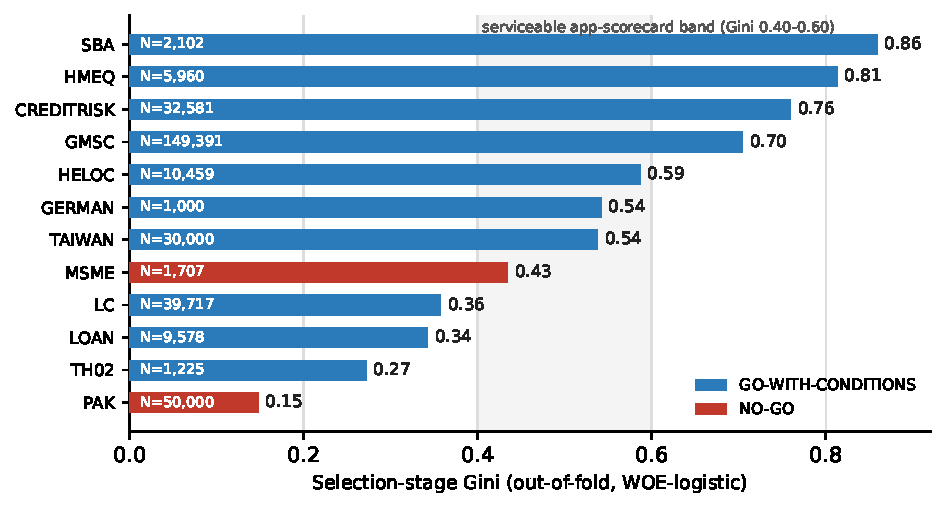
\includegraphics[width=\linewidth]{corpus_gini.pdf}
\caption{Selection-stage Gini across the governed corpus, coloured by sealed GF verdict.
Discrimination spans an order of magnitude; the two NO-GO runs are not simply the
lowest-Gini---MSME is rejected on sufficiency, not discrimination.}
\label{fig:corpus}
\end{figure}

\subsection{A worked run: German credit, G0 to GF}
To make the pipeline concrete, we trace one dataset end-to-end. On German credit
($N{=}1{,}000$, $30\%$ default rate), \textbf{G0} excludes the three protected attributes
(age, sex/marital status, foreign-worker status) and sets a \textsc{medium} materiality tier,
leaving a 17-feature pool. \textbf{G1} accepts the univariate screen---12 of 17 features pass,
and both sufficiency diagnostics are met (EPV ${\approx}17.6$; Riley minimum $323$ vs $1{,}000$
available)---with \texttt{checking\_status} dominant (IV $0.67$). \textbf{G2} confirms all 12
players above the shadow-feature null; the U-shaped \texttt{credit\_amount}, which a monotonic
IV screen under-rates, is vindicated at the model check and enters the selected set. \textbf{G3}
selects $k{=}5$ features
(\texttt{checking\_status}, \texttt{credit\_history}, \texttt{months\_duration},
\texttt{savings\_status}, \texttt{credit\_amount}), Gini $0.54$---the smallest $k$ at which the
equivalence test ($p{=}0.11$) and the $5\%$ tolerance ($4.6\%$) clear \emph{together}.
\textbf{G4} finds calibration sound (Hosmer--Lemeshow $p{=}0.11$, ECE $0.03$) and fairness
mixed: the sex adverse-impact ratio is clean ($0.93$) while the age ratio fails four-fifths
($0.34$) \emph{despite age being excluded}---a true-risk-driven disparity reconstructed through
correlated features. \textbf{G5} fixes the scoring controls (mandatory \texttt{checking\_status};
exact reason codes; PD floor), and \textbf{GF} rules GO-WITH-CONDITIONS. Every decision is
signed and appended to the hash chain, which seals at a final digest; an independent re-run
reproduced every gate and the chain exactly (\S\ref{sec:setup}).

\subsection{Parsimony varies with sample size}
The single fixed stopping rule (\ref{eq:stop}) produces strikingly different parsimony
depending on $N$, because DeLong's power to detect the loss from dropping a weak feature grows
with sample size. At \textbf{small $N$} the rule genuinely parsimonises: on German
($N{=}1{,}000$) it selects $5$ of $17$ features, with both conditions clearing together
(DeLong $p{=}0.107\ge0.05$ and relative-Gini loss $4.56\%\le5\%$). At \textbf{large $N$} the
same rule returns a near-full set: on LC ($N{\approx}40{,}000$) it keeps $8$ of $9$ players
(DeLong $p{=}1.0$, loss $0.0\%$), and on HMEQ ($N{\approx}6{,}000$) DeLong rejects \emph{every}
proper subset ($k{=}9$ vs full, $p{=}6.1\times10^{-4}$) even though a $5\%$-loss criterion alone
would admit a six-feature model---so the \emph{and}-rule returns all eleven. This is the
methodology declining to overstate parsimony when the data can resolve the difference. We call
this a \emph{large-sample significance effect}: the same rule, opposite behaviour at the two ends of the
sample-size range, both honest. A corollary visible in Table~\ref{tab:corpus} is that
\emph{signal, not volume, sets the ceiling} (Fig.~\ref{fig:signalvol})---German reaches Gini
$0.54$ on $1{,}000$ rows while LC reaches $0.36$ on $40{,}000$.

\begin{figure}[!t]
\centering
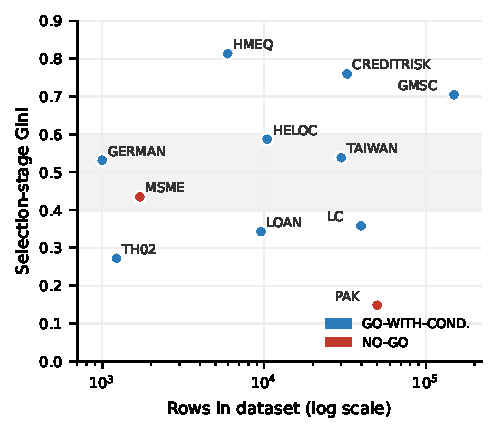
\includegraphics[width=0.84\linewidth]{fig_signal_volume.pdf}
\caption{Signal, not volume, sets the ceiling: each dataset's selection-stage Gini against its
sample size (log scale), coloured by sealed verdict. More rows do not raise the achievable
discrimination---German ($1{,}000$ rows) outscores LC ($40{,}000$) and GMSC ($149{,}391$).}
\label{fig:signalvol}
\end{figure}

\subsection{Fairness: excluding a protected attribute is necessary but not sufficient}
Fairness is identified by a fixed \emph{proxy-leakage} procedure: we partition the held-out set by a
protected attribute the model \emph{does not use}, take the model's favourable-decision rate per group
on the internal master scale (indicative---no institution cutoff), and report the adverse-impact ratio
against the four-fifths rule; where a group fails, we test whether the model is accurate \emph{within}
each group, which separates true-risk-driven disparity from proxy bias.
On two independent datasets, removing the protected attribute did not remove disparate impact,
because correlated features reconstruct it. On \textbf{LC}, geography (\texttt{addr\_state}) was
dropped at a cost of only $0.007$ Gini, yet a residual regional approve-rate disparity persisted
(worst adverse-impact ratio $0.62$, below the four-fifths bar). On \textbf{German}, \texttt{age}
was excluded at G0, yet the age-band approve-rate AIR was $0.34$ (under-25 default rate $41.3\%$
vs $25.5\%$ for $60+$); because the model is accurate \emph{within} each band, this is disparate
\emph{impact driven by true risk}, not proxy bias. Both runs therefore record the same governed
finding (Fig.~\ref{fig:air})---proxy removal is necessary but not sufficient, and a
fairness-constrained replication or reject-inference study would be required before any live
use---surfaced as a binding GF condition rather than discovered post-deployment.

\begin{figure}[!t]
\centering
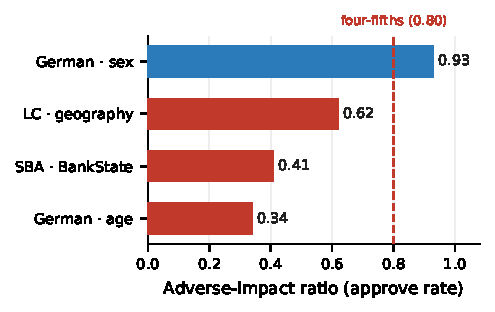
\includegraphics[width=0.84\linewidth]{fig_fairness_air.pdf}
\caption{Adverse-impact ratio after the protected attribute is excluded, against the four-fifths
bar ($0.80$). Sex is clean; age (German) and geography (LC, SBA) fail despite the attribute being
excluded---disparate impact reconstructed through correlated features, true-risk-driven in each
case.}
\label{fig:air}
\end{figure}

\subsection{Calibration}
With class reweighting off and isotonic calibration always on, calibrated probabilities are
tight across the corpus: expected calibration error is $0.020$ on HMEQ, $0.002$ on LC,
$0.033$ on German and $0.007$ on MORTGAGE, and Hosmer--Lemeshow is \emph{not} rejected even at the
largest $N$ (GMSC $149{,}391$, LC). The one exception is the origination-only MORTGAGE model
($N{=}50{,}049$), where HL \emph{is} rejected at $g{=}10$ ($p{\approx}0$) but passes at $g{=}5$
($p{=}0.34$) with the per-grade backtest clean ($8/8$ grades inside the Wilson interval): the
large-$N$ hypersensitivity that dominates parsimony surfaces for calibration only on the coarsest-
fitting model, and there the per-grade realised-vs-expected backtest---not HL---is the governing
test (as recorded at G4 for that run). \emph{Which backtest.} The per-grade backtests sealed for the fourteen corpus runs were computed on
out-of-fold predictions. A stricter variant, which fits the isotonic calibrator on one part of the data
and tests the \emph{deployed} calibrated model on a held-out part, was introduced later (first with
the mortgage hazard framing) and is used in \S\ref{sec:polish1}; the earlier runs have not yet been
re-verified under it, so the two are not directly comparable. Because the learner is WOE-logistic, each
PD carries an exact additive reason-code decomposition. Fig.~\ref{fig:reliability} illustrates the per-grade reliability on CREDITRISK,
whose model spans the full AAA--D range: observed default rates track the predicted probabilities
closely across nearly two orders of magnitude.

\begin{figure}[!t]
\centering
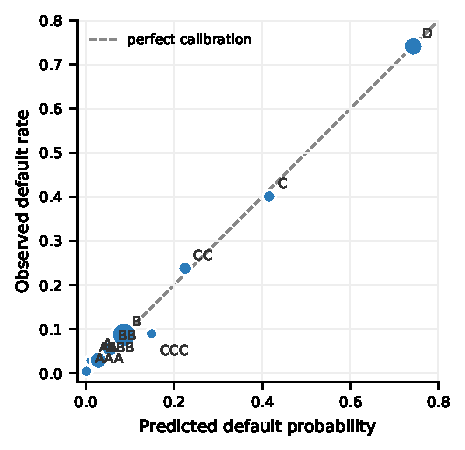
\includegraphics[width=0.74\linewidth]{reliability.pdf}
\caption{Per-grade calibration reliability on the CREDITRISK held-out set (rating grades AAA--D;
marker area $\propto$ grade population). Points lie close to the diagonal across the full risk
range; Hosmer--Lemeshow is not rejected ($p{=}0.44$, ECE $0.011$). The one mild outlier is the
small \textsc{ccc} grade, which over-predicts (a conservative direction).}
\label{fig:reliability}
\end{figure}

\subsection{Sample-size adequacy (EPV and Riley)}
Table~\ref{tab:riley} reports the two sufficiency diagnostics on two bases. Riley's parameter count $P$ is
the number of candidate parameters considered \emph{before} data-driven selection, so the governing basis is the
candidate pool; the selected-feature count, which an earlier version of this analysis used, is shown beside it.
Screening by information value, Shapley confirmation and parsimony selection all use the outcome, so a count reduced
by them cannot lower the requirement. On the pool basis twelve of fourteen runs meet the Riley minimum. \textbf{MSME}
is short (requires $21{,}200$, has $1{,}707$; on the selected basis $3{,}654$) and fails \emph{both} diagnostics---it is the
only HIGH-tier NO-GO, so the clearest failure is the case already rejected. \textbf{TH02} is also short on the pool
basis (requires $2{,}731$, has $1{,}225$) although it passed by $55$ rows on the selected basis; its sealed verdict
was not altered, because sufficiency is a reported diagnostic and never an automatic rejection. The two diagnostics
diverge in both directions, which is Riley's value over EPV. Below EPV $10$ on the pool basis sit \textbf{POLISH-5y}
($4.2$) and MSME ($1.2$); POLISH-5y nonetheless meets Riley ($5{,}555$ against $7{,}027$) because its strong signal
(Gini $0.78$) clears the shrinkage criterion despite thin events ($271$). The converse is \textbf{PAK}, whose
EPV is enormous yet which needs $26{,}262$ rows on the pool basis because its weak signal (AUC
$0.57\Rightarrow R^2_{cs}{=}0.013$) makes shrinkage demand volume.
Fig.~\ref{fig:riley} shows the headroom as rows available over rows required.

\begin{figure}[!t]
\centering
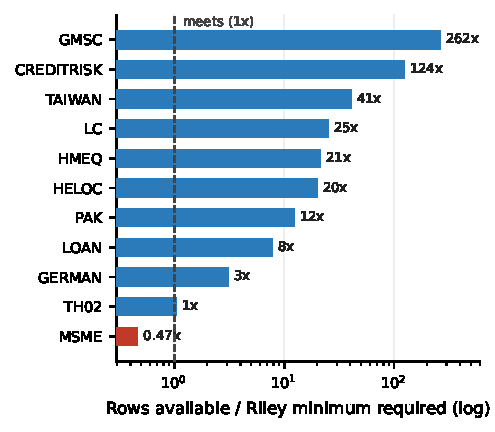
\includegraphics[width=0.84\linewidth]{fig_riley_headroom.pdf}
\caption{Sample-size headroom on the governing (candidate-pool) basis: rows available divided by the Riley
minimum required (log scale; dashed line is the $1\times$ meets-the-minimum point). MSME ($0.08\times$) and TH02
($0.45\times$) fall short; PAK clears by $1.9\times$ despite a huge EPV, because its weak signal raises the
requirement.}
\label{fig:riley}
\end{figure}

\begin{table}[!t]
\centering
\caption{Riley minimum-$N$ retrospective (reported diagnostic), $N_{\text{req}}=\max(B1,B3,B4)$. The
\emph{pool} columns are the governing basis: $P$ is the candidate pool (columns entering Stage~1 after
eligibility), because selection that uses the outcome cannot lower the requirement. The selected-$P$ columns
are the earlier basis. Meets? refers to the pool basis.}
\label{tab:riley}
\footnotesize
\setlength{\tabcolsep}{2.5pt}
\begin{tabular}{@{}lrrrrrl@{}}
\toprule
Dataset & $N$ & $N_{\text{req}}^{\text{sel}}$ & $N_{\text{req}}^{\text{pool}}$ & EPV$^{\text{sel}}$ & EPV$^{\text{pool}}$ & Meets? \\
\midrule
SBA        & 2{,}102 & 338 & 380 & 62 & 36.1 & yes \\
HMEQ       & 5{,}960 & 278 & 304 & 108 & 99.1 & yes \\
POLISH-5y  & 7{,}027 & 3{,}212 & 5{,}555 & 7.3 & 4.2 & yes \\
CREDITRISK & 32{,}581 & 263 & 263 & 1185 & 790 & yes \\
GMSC       & 149{,}391 & 570 & 642 & 1251 & 1112 & yes \\
HELOC      & 10{,}459 & 522 & 706 & 321 & 237 & yes \\
TAIWAN     & 30{,}000 & 737 & 1{,}052 & 474 & 332 & yes \\
GERMAN     & 1{,}000 & 323 & 760 & 60 & 17.6 & yes \\
MORTGAGE   & 50{,}049 & 358 & 597 & 2526 & 1516 & yes \\
MSME       & 1{,}707 & 3{,}654 & 21{,}200 & 6.8 & 1.2 & \textbf{no} \\
LC         & 39{,}717 & 1{,}581 & 3{,}690 & 625 & 268 & yes \\
LOAN       & 9{,}578 & 1{,}220 & 2{,}267 & 219 & 118 & yes \\
TH02       & 1{,}225 & 1{,}170 & 2{,}731 & 54 & 23.1 & \textbf{no} \\
PAK        & 50{,}000 & 4{,}041 & 26{,}262 & 2173 & 334 & yes \\
\bottomrule
\end{tabular}

\vspace{2pt}
{\footnotesize POLISH-5y's earlier entry ($5{,}141$) used $P{=}60$, the screened count, not the selected count of the
other rows; on the selected basis it is $3{,}212$. Requirements vary by about $\pm2$ between the selected column
here and the original table because the $R^2_{cs}$ simulation is seeded on rounded inputs. The pool figure uses the
selected model's C-statistic, because the pool model is never fitted.\par}
\end{table}

\subsection{A staged run: Polish bankruptcy, one year ahead}\label{sec:polish1}
The Polish file whose outcome is checked one year ahead (5{,}910 firms, 410 bankruptcies, 6.94\%; 64
financial ratios; seed $42$, same fixed configuration) was the first dataset run under the staged
protocol, with every gate signed before the next stage ran. It is not part of Table~\ref{tab:corpus}:
its firms and event rate differ from the five-year-ahead file, so the two are not a paired comparison, and
no test of whether discrimination falls with horizon has been made.

Screening passes $63$ of $64$ ratios (the dominant ratio, sales growth, has information value $2.19$).
Attribution confirms $19$ players above the shadow bar ($0.00161$; weakest $1.74\times$). Selection
chooses $k{=}4$ players spanning $25$ columns: Gini $0.826$ (95\% CI $0.797$--$0.857$) against $0.838$ for
the full set, DeLong $p{=}0.255$, relative loss $1.4\%$. EPV is $6.4$ on the candidate pool and $16.4$ on the
selected model, which meets the Riley minimum with a $5.2\times$ margin. The deployed-model backtest passes
$9$ of $10$ grades on $1{,}182$ held-out firms; grade~B under-predicts risk ($16.7\%$ realised against
$8.3\%$ expected), and Hosmer--Lemeshow does not reject with ten groups ($p{=}0.072$) but rejects with five
($p{=}0.019$). The sealed verdict is GO-WITH-CONDITIONS.

The run also shows what the staged reports are for. The ratio `sales growth' is blank for $103$ firms,
$99$ of them bankrupt ($96.1\%$; Fisher $p<10^{-100}$), so a model that scores a blank as a value assigns
those firms near-certain default. The pattern is a data-collection artefact of unknown cause, not a financial
ratio, and it was noticed only at the deployment gate because the blank-versus-outcome scan did not yet
exist; with the scan it appears at G0. The deployed control refers a blank application instead of scoring it.
On complete rows the in-sample AUC is $0.895$ against $0.920$ on all rows (descriptive, not out-of-fold), so part of the
reported discrimination rests on the pattern. Two further items stay open: one profitability ratio is defined
over `gross profit in 3 years', and the source does not say whether those years follow the statement date; and
bankrupt and operating firms were sampled in different calendar windows. The acceptance pack exercised the PD floor
but never the $99.9\%$ cap (the highest PD among scored firms is well below it), and one real bankrupt firm is
rated in the best grade.

\section{Discussion}\label{sec:discussion}
\textbf{Governance without contaminating the analytics.} The central design choice---that gates
decide scope, eligibility, fairness treatment and disposition but never the analytical method
(P8)---is what makes the corpus comparable at all. Because the estimator, tolerances, shadow bar
and seed are fixed across every dataset, a difference in outcome is a property of the data, not
of a per-run tuning decision. The governance layer buys traceability and accountability; it does
not buy, and must not buy, the freedom to change the method until the answer improves.

\textbf{What the findings mean for practice.} This large-sample effect is not a defect of the
rule but a faithful consequence of it: at large $N$ a paired-AUC test can resolve the loss from
dropping even a weak feature, so an honest equivalence criterion returns a fuller model.
Practitioners should therefore expect genuine parsimony mainly at modest sample sizes and treat a
large-$N$ ``parsimonious'' claim with suspicion. The fairness result sharpens a familiar warning:
because correlated features reconstruct an excluded attribute, proxy removal is a floor, not a
remedy, and the responsible posture is to \emph{measure and disclose} residual disparate impact
(here as an indicative adverse-impact ratio, with the accept/decline cutoff left exogenous) and
bind a fairness-constrained follow-up, rather than to claim fairness by omission.

\textbf{Limitations.} This study validates a \emph{procedure}, not a performance claim: we do not
yet assert that the methodology selects better subsets than established alternatives---that requires the
pre-specified benchmark against LASSO, elastic net, RFE, Boruta and TreeSHAP, which is
implemented but not run across the corpus. Validation of the corpus runs is i.i.d.\ cross-validation; none is evaluated out of time, so no
out-of-time or production-readiness claim is made. All datasets are
accept-only samples, so feature effects are subject to range restriction \cite{handhenley1997}.
The governance roles are exercised by a single researcher in this methodological setting; the
framework specifies the \emph{structure} of independent challenge rather than demonstrating a multi-party
deployment. In the staged Polish run the researcher chose every option, but the rationale text was drafted
by an AI assistant, shown before sealing, and recorded as such; the independence rows of the acceptance
checklist (R7, R8) are therefore partial. The Polish run also leaves two data questions open (a possible
look-ahead in one ratio and a sampling-window confound between bankrupt and operating firms), and its
discrimination partly rests on a blank-value pattern whose cause is unknown (\S\ref{sec:polish1}). Finally, the Riley diagnostic is governed on the candidate pool, and the pool model is never
fitted, so the selected model's C-statistic stands in for the anticipated one; the closed-form approximation can also
under-state the requirement at very high $C$. Sufficiency is a reported diagnostic and altered no verdict, including
the pool-basis shortfall of TH02; both points are disclosed.

\section{Future Work}\label{sec:future}
Several directions follow directly from the limitations above.
\emph{Comparative evaluation.} The pre-specified benchmark against LASSO, elastic net, recursive
feature elimination, Boruta and TreeSHAP---implemented but not yet run across the corpus---will
test whether the methodology selects \emph{better} subsets than established alternatives,
upgrading the present ``defensible'' claim to a comparative one.
\emph{Temporal validation.} An exploratory discrete-time (hazard) analysis of the mortgage panel
with an out-of-time split exists outside the reported corpus; extending it, and applying the pipeline to
other datasets with a reliable time index, would support out-of-time validation and a survival /
competing-risks extension, replacing the current
i.i.d.\ cross-validation scope and supporting a production-readiness claim.
\emph{Reject inference.} Because all datasets are accept-only, incorporating reject inference would
correct the range restriction that attenuates feature effects, and would sharpen the fairness
analysis in particular.
\emph{Fairness-constrained selection.} Since excluding a protected attribute does not remove
disparate impact, a natural extension searches for a less-discriminatory alternative---through
fairness-constrained selection or a penalised objective---and reports the discrimination cost of
each constraint, making the fairness trade-off an explicit, governed decision.
\emph{Multi-party governance.} Exercising the role separation with genuinely independent signers,
integrated with a live model-risk workflow, would let us measure the governance overhead and the
framework's effect on validation turnaround.
\emph{Sample-size refinement.} For high-discrimination settings where the closed-form Riley bound
can under-state the requirement, a simulation-based minimum sample size and a candidate-pool
parameter count would tighten the reported sufficiency diagnostic.

\section{Conclusion}\label{sec:conclusion}
We have presented a pre-registered feature-selection methodology that separates
Shapley attribution from an explicit parsimony rule and reports its own calibration, fairness and
sample-size adequacy, wrapped in a hash-chained, materiality-tiered governance framework that
records who decided what, on what evidence, and under which cited bar. Run as one fixed
configuration across fourteen credit datasets, the pair surfaces findings that analyst discretion
would obscure---sample-size-dependent parsimony, disparate impact that survives protected-attribute
removal, and the primacy of signal over volume---while inventing no economic assumptions:
thresholds and pricing remain institution inputs. We hope the reproducible, auditable discipline demonstrated
here lowers the cost of independent model validation and raises the bar for what counts as a
defensible credit model.

\section*{Appendix: Reproducibility}
The configuration is fixed across every dataset and chosen once (Table~\ref{tab:config}), with the
random seed $42$ throughout, and no governance gate re-opens any of it (P8). Reproducibility rests
on this fixed configuration together with the determinism of the pipeline: independent re-runs of
two datasets reproduced their committed results exactly (\S\ref{sec:setup}). Each gate decision is
additionally recorded in an append-only, hash-chained log (\S\ref{sec:aegis}, Eq.~\ref{eq:hash})
so that any later edit to a sealed record is detectable; the per-run decision logs accompany the
paper's artefact. For staged runs the artefact also holds the chain and the stage outputs of each run, and an
automated test checks that the staged runner reproduces the one-shot pipeline.

\begin{table}[!t]
\centering
\caption{The fixed configuration (identical for every dataset; seed $42$).}
\label{tab:config}
\footnotesize
\begin{tabular}{@{}p{0.42\linewidth}p{0.5\linewidth}@{}}
\toprule
Parameter & Value \\
\midrule
Learner (all stages) & WOE-logistic \\
Value function & cross-validated AUC \\
Correlation grouping & single player at $|\rho|\ge0.7$ \\
Shadow players & $\ge10$; bar $=$ 95th percentile \\
Confirmation frequency & $\ge0.80$ \\
Exact vs sampled Shapley & exact if players $\le15$, else sampled \\
Selection rule & smallest $k$: DeLong $p\ge0.05$ \emph{and} rel.\ Gini loss $\le5\%$ \\
Calibration & isotonic, 5-fold \\
PD floor / cap & $0.03\%$ / $99.9\%$ \\
Split & stratified $80/20$ pre-resampling; 5-fold OOF \\
Random seed & $42$ \\
\bottomrule
\end{tabular}
\end{table}

\bibliographystyle{IEEEtran}
\bibliography{refs}

\end{document}
